\documentclass{standalone}
\usepackage{pgfplots}
\usetikzlibrary{intersections}
\usepgfplotslibrary{fillbetween}
\pgfplotsset{compat=1.7}

\begin{document}
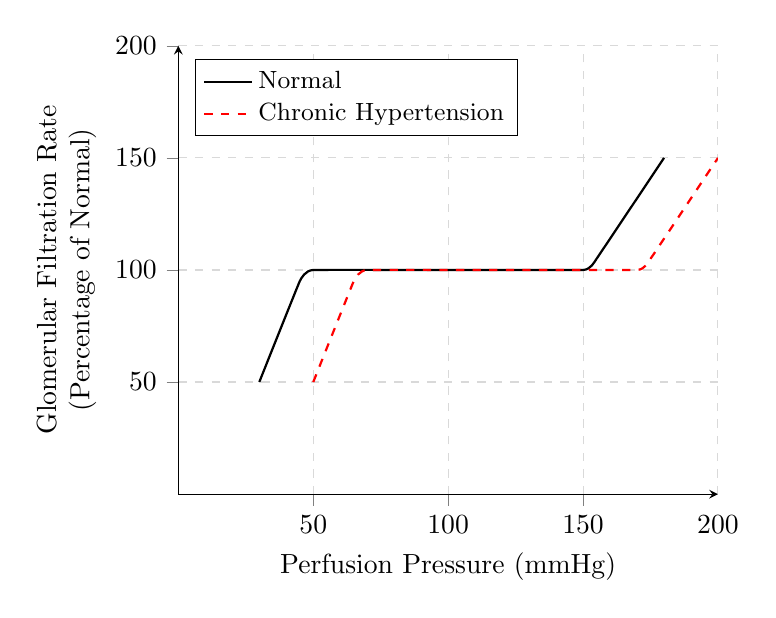
\begin{tikzpicture}


\begin{axis}[
        axis lines=middle,
        grid = major,
        grid style={dashed, gray!30},
	ymin = 0,
	ymax = 200,
	xmin = 0,
	xmax =200,
	 ylabel near ticks,
	xlabel near ticks,
        xlabel=Perfusion Pressure (mmHg),
        ylabel=Glomerular Filtration Rate \\ (Percentage of Normal),
        tick align=outside,
        enlargelimits=false,
ylabel style={align=center},
legend pos= north west,
legend style={font=\small, cells={align=left}},
legend cell align={left}]

\draw[black, thick] plot[smooth,tension=0.1] coordinates { (axis cs: 30,50) (axis cs: 45,95) (axis cs: 50,100) (axis cs: 150,100) (axis cs: 155,105) (axis cs: 180,150)};
\draw[red,dashed, thick] plot[smooth,tension=0.1] coordinates { (axis cs: 50,50) (axis cs: 65,95) (axis cs: 70,100) (axis cs: 170,100) (axis cs: 175,105) (axis cs: 200,150)};

\addplot[black, thick]{-1};
\addplot[red,dashed,thick]{-1};
\addlegendentry{Normal};
\addlegendentry{Chronic Hypertension};

\end{axis}

\end{tikzpicture} 
\end{document}